\documentclass[aspectratio=169,11pt]{beamer}

\usepackage{graphicx}
\usepackage{tikz}
\usetikzlibrary{positioning,arrows.meta}
\usepackage{xcolor}  
\usepackage{booktabs}
\usepackage{tabularx}
\usepackage{array}
\usepackage{ragged2e}

\definecolor{GEUBlue}{RGB}{20,55,105}
\definecolor{GEULightBlue}{RGB}{238,244,251}
\definecolor{GEUGrey}{RGB}{90,90,90}
\definecolor{GEULightGrey}{RGB}{245,246,248}

\usetheme{default}
\setbeamertemplate{navigation symbols}{}
\setbeamertemplate{blocks}[rounded][shadow=false]
\setbeamercolor{normal text}{fg=black,bg=white}
\setbeamercolor{frametitle}{fg=GEUBlue}
\setbeamercolor{structure}{fg=GEUBlue}
\setbeamercolor{block title}{fg=GEUBlue,bg=GEULightBlue}
\setbeamercolor{block body}{fg=black,bg=GEULightBlue}
\setbeamerfont{frametitle}{size=\Large,series=\bfseries}

% Replace with the actual logo filename
\newcommand{\GEULogo}{graphicera_logo.png}

% Header and footer
\setbeamertemplate{headline}{%
  \begin{tikzpicture}[remember picture,overlay]
    \node[anchor=north east,xshift=-0.30cm,yshift=-0.12cm]
      at (current page.north east)
      {\includegraphics[height=0.62cm]{\GEULogo}};
  \end{tikzpicture}
  \vspace{0.72cm}
}
\setbeamertemplate{frametitle}{%
  \vspace{-0.2cm}
  \insertframetitle\par
  \vspace{0.02cm}
  \textcolor{GEUBlue}{\rule{\textwidth}{0.9pt}}
  \vspace{-0.12cm}
}
\setbeamertemplate{footline}{%
  \leavevmode
  \hbox{%
  \begin{beamercolorbox}[wd=.82\paperwidth,ht=0.32cm,dp=0.10cm,leftskip=.3cm]{author in head/foot}
    \tiny Department of Computer Science \& Engineering | Graphic Era (Deemed to be University)
  \end{beamercolorbox}%
  \begin{beamercolorbox}[wd=.18\paperwidth,ht=0.32cm,dp=0.10cm,rightskip=.3cm]{date in head/foot}
    \hfill\tiny\insertframenumber/\inserttotalframenumber
  \end{beamercolorbox}}
}

\newcommand{\smallnote}[1]{\vspace{0.08cm}{\scriptsize\color{GEUGrey}#1}}
\newcommand{\placeholder}[1]{\textit{\color{GEUGrey}#1}}
\title{\textbf{Project-Based Learning}\\[2mm]\large Phase-I Evaluation}
\author{\textbf{FOOD RESCUE -- Smart Food Rescue and Redistribution System}\\Team ID: DSCPP-III-2026-T381}
\institute{Department of Computer Science \& Engineering\\Graphic Era (Deemed to be University), Dehradun}
\date{Academic Session 2026--27}

\begin{document}

% 1
\begin{frame}[plain]
\begin{tikzpicture}[remember picture,overlay]
\draw[GEUBlue,line width=3pt] (current page.north west) -- (current page.north east);
\node[anchor=north east,xshift=-0.45cm,yshift=-0.35cm] at (current page.north east)
{\includegraphics[height=1.0cm]{\GEULogo}};
\node[align=center,text width=.84\paperwidth] at ([yshift=.25cm]current page.center)
{{\color{GEUBlue}\fontsize{26}{30}\selectfont\bfseries PROJECT-BASED LEARNING}\\[3mm]
 {\fontsize{18}{22}\selectfont PHASE-I EVALUATION}\\[7mm]
 {\color{GEUGrey}\Large\bfseries FOOD RESCUE\\\normalsize Smart Food Rescue and Redistribution System}\\[3mm]
 {\color{GEUBlue}\normalsize Team ID: DSCPP-III-2026-T381}};
\node[align=center,anchor=south,yshift=.42cm] at (current page.south)
{\bfseries Department of Computer Science \& Engineering\\
Graphic Era (Deemed to be University), Dehradun\\[-1mm]
\scriptsize Academic Session 2026--27};
\end{tikzpicture}
\end{frame}

% 2
\begin{frame}{Team \& Mentor Details}
\begin{columns}[T,totalwidth=\textwidth]
\column{.42\textwidth}
\begin{block}{Team Information}
\scriptsize
\begin{tabular}{@{}ll@{}}
\textbf{Team ID:} & DSCPP-III-2026-T381 \\
\textbf{section:} & ML2 , ML3 , DS1 , ML4 \\
\textbf{Semester:} & 3rd\\
\textbf{Domain:} & SOCIAL IMPACT 
\end{tabular}
\end{block}
\column{.5\textwidth}
\begin{block}{Team Members}
1.\quad ADITYA DUTTA (Lead) -- 2510373905\\
2.\quad UTSAV BAJORIA -- 2510370581\\
3.\quad VISHWAJEET SINGH -- 2510380298\\
4.\quad RAGHAV PANDEY -- 2510380113\\
\end{block}
\end{columns}
\vspace{2mm}
\begin{block}{Mentor}
Mr. CHIRAG TYAGI
\hfill
\textbf{Interactions completed:} 5
\end{block}
\end{frame}

% 3
\begin{frame}{Problem Statement \& Motivation}
\begin{block}{Problem Statement}
\footnotesize Restaurants, hostels, households, and events often generate surplus food that is still safe to consume, while NGOs and people in need may face shortages. Without proper coordination, this usable food goes to waste. FoodRescue connects donors with NGOs, recording food quantity, location, type, and expiry, and prioritizing by expiry, quantity, and distance.
\end{block}
\vspace{1mm}
\begin{columns}[T,totalwidth=\textwidth]
\column{.48\textwidth}
\footnotesize
\textbf{\color{GEUBlue}Motivation}
\begin{itemize}\itemsep1pt
\item Restaurants, hostels, households, and events generate surplus food that's still safe to eat
\item Without proper coordination, this usable food simply goes to waste
\item NGOs and people in need often face shortages at the same time
\end{itemize}
\column{.48\textwidth}
\footnotesize
\textbf{\color{GEUBlue}Target Users / Stakeholders}
\begin{itemize}\itemsep1pt
\item Food donors: restaurants, hostels, households, event organizers
\item NGOs and people in need (recipients)
\item Volunteers responsible for delivery
\end{itemize}
\end{columns}
\end{frame}



% 4
\begin{frame}{Objectives}
\textbf{\color{GEUBlue}Project Objectives}
\vspace{2mm}
\begin{enumerate}\itemsep5pt
\item understand the requirements and design the main entities and classes.
\item manage donors, food donations, requirements, and volunteers.
\item select donations by priority and match donors with NGOs.
\item design graph of location and find the best delivery route using Dijkstra's algorithm.
\item Add delivery tracking, test system and check whether food getting delivered to people in need or not.
\end{enumerate}
\vfill
\begin{center}
\colorbox{GEULightBlue}{\parbox{.80\textwidth}{\centering
\textbf{Key Objective:} A working C++ (OOP + DSA) system connecting food donors with NGOs for redistribution.}}
\end{center}
\end{frame}

% 5
\begin{frame}{Proposed Solution}
\begin{columns}[T,totalwidth=\textwidth]
\column{.48\textwidth}
\small
\textbf{\color{GEUBlue}Proposed Approach}
\begin{enumerate}\itemsep2pt
\item Donor registers a \texttt{FoodDonation} (type, qty, expiry, location)
\item Priority queue ranks urgency; queue handles NGO requests
\item Hash table: fast donor/NGO/volunteer lookup
\item Graph + Dijkstra's algorithm: best delivery route
\item Delivery tracked from registration to drop-off
\end{enumerate}
\column{.48\textwidth}
\small
\textbf{\color{GEUBlue}Key Features}
\begin{itemize}\itemsep2pt
\item Web front-end (HTML/CSS/JS) for all 3 roles
\item C++ backend: Donor, FoodDonation, NGO, Volunteer, Requirement, Delivery classes
\item Priority-based donation selection \& matching
\item Dijkstra-based route planning
\item Delivery tracking + file-based storage
\end{itemize}
\end{columns}
\vfill
\end{frame}

% 6
\begin{frame}{Integration of PBL Course Concepts}
\scriptsize
\begin{center}
\renewcommand{\arraystretch}{1.25}
\begin{tabularx}{.96\textwidth}{@{}>{\bfseries}p{3.0cm}X p{2.5cm}@{}}
\toprule
Course & Concepts Applied & Project Module\\
\midrule
Data Structures in C & Priority queue for urgent-donations; using queue for NGO requests; we are using hash table for fast donor/NGO/volunteer lookup; Graph and Dijkstra's algorithm together for better delivery route & DSA-Based Matching \& Optimization Layer\\
OOPs with C++ & Classes: Donor, FoodDonation, NGO, Volunteer, Requirement, Delivery; Inheritance \& Polymorphism for role-specific behavior; STL containers; File handling for persistence & Application / Data Management Layer\\
\bottomrule
\end{tabularx}
\end{center}
\vfill
\begin{center}
\colorbox{GEULightBlue}{\parbox{.86\textwidth}{\centering
\textbf{Requirement:} Demonstrate meaningful integration of both subjects in \textbf{one} project.}}
\end{center}
\end{frame}

% 7: System Architecture / Workflow
\begin{frame}{System Architecture / Workflow}
\begin{center}
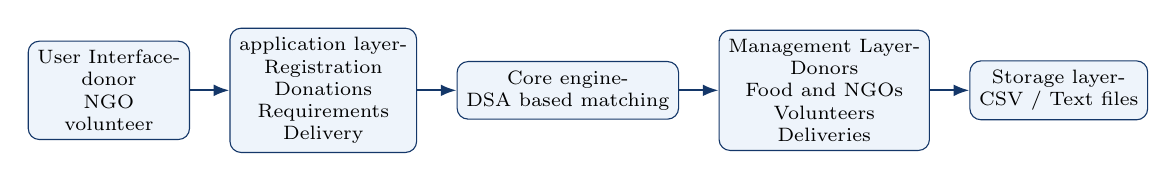
\begin{tikzpicture}[
node distance=5mm,
box/.style={rectangle,rounded corners,draw=GEUBlue,fill=GEULightBlue,
minimum width=1cm,minimum height=5mm,align=center,font=\scriptsize},
arrow/.style={-{Latex[length=2mm]},thick,draw=GEUBlue}
]
\node[box] (a) {User Interface-\\donor\\NGO\\volunteer};
\node[box,right=of a] (b) {application layer-\\Registration\\ Donations\\Requirements\\Delivery};
\node[box,right=of b] (c) {Core engine-\\DSA based matching};
\node[box,right=of c] (d) {Management Layer-\\Donors\\Food and NGOs\\ Volunteers\\Deliveries};
\node[box,right=of d] (e) {Storage layer-\\ CSV / Text files};
\draw[arrow] (a)--(b); \draw[arrow] (b)--(c); \draw[arrow] (c)--(d); \draw[arrow] (d)--(e);
\end{tikzpicture}
\end{center}
\vspace{2mm}
\begin{columns}[T,totalwidth=\textwidth]
\column{.48\textwidth}
\textbf{\color{GEUBlue}Major Components}
\begin{itemize}\itemsep2pt
\item \textbf{UI Layer:} Donors,NGO's,volunteers interact with online system.
\item \textbf{Logic Engine:} Constraint checker \& allocation logic.
\item \textbf{Data Management:} keeps track of all donor, NGO, volunteer & delivery records
\end{itemize}
\column{.48\textwidth}
\textbf{\color{GEUBlue}Data / Control Flow}
\footnotesize
\begin{itemize}\itemsep1pt
\item Donor lists a food donation (type, qty, expiry, location)
\item Engine ranks by urgency, matches to a suitable NGO, routes via Dijkstra's algorithm
\item Volunteer assigned; delivery tracked to storage
\end{itemize}
\end{columns}
\end{frame}


% 8
\begin{frame}{Technology Stack \& Methodology}
\begin{columns}[T,totalwidth=\textwidth]
\column{.48\textwidth}
\begin{block}{Technology Stack}
\begin{itemize}\itemsep2pt
\item Backend: C++ (STL, OOP, DSA)
\item Frontend: HTML, CSS, JavaScript
\item Storage: File-based (CSV / Text records)
\item Tools / Framework: Standard Template Library (STL)
\item IDE: VS Code / Code::Blocks 
\item Version Control: Git / GitHub
\end{itemize}
\end{block}
\column{.48\textwidth}
\begin{block}{Development Methodology}
\begin{enumerate}\itemsep2pt
\item Requirement Analysis
\item System Design
\item Implementation
\item Testing
\item Evaluation
\end{enumerate}
\end{block}
\end{columns}
\vfill
\begin{center}
\end{center}
\end{frame}

% 9
\begin{frame}{Initial Progress \& Team Contribution}
\begin{columns}[T,totalwidth=\textwidth]
\column{.44\textwidth}
\textbf{\color{GEUBlue}Progress Achieved}
\begin{itemize}\itemsep3pt
\item Literature/background study on food-rescue platforms completed
\item Requirements and user roles finalized
\item System architecture and class diagram prepared
\end{itemize}
\column{.52\textwidth}
\textbf{\color{GEUBlue}Individual Contribution}
\vspace{2mm}
\small
\begin{tabularx}{\textwidth}{@{}p{2.6cm}X@{}}
\toprule
Member & Module\\
\midrule
Aditya Dutta & Core-DSA, Integration \& UI \\
Utsav Bajoria & Volunteer \& Delivery Module \\
Vishwajeet Singh & NGO \& Requirement Module \\
Raghav Pandey &Donor \& Food Donation Module \\
\bottomrule
\end{tabularx}
\end{columns}
\end{frame}

\begin{frame}{Roadmap, Expected Outcomes \& References}
\begin{columns}[T,totalwidth=\textwidth]
\column{.55\textwidth}
\textbf{\color{GEUBlue}Roadmap}
\begin{enumerate}\itemsep3pt
\item Requirements \& core entity/class design
\item Donor, volunteer management
\item Priority-based selection 
\item best delivery route
\item Delivery tracking \& testing
\end{enumerate}
\vspace{1mm}
\textbf{\color{GEUBlue}Expected Outcomes}
\begin{itemize}\itemsep2pt
\item {automated priority based matching}
\item {To cut food wastage and get surplus meals to people who need them}
\item {GPS backed mobile platform serving multiple cities and NGO's}
\end{itemize}
\column{.47\textwidth}
\textbf{\color{GEUBlue}References}
\begin{enumerate}\itemsep3pt
\item Cormen, T.H.,Leiserson,C.E.,Rivest,R.L.,and Stein,C. -- \textit{Introduction to Algorithms}
\item Balagurusamy, E. -- \textit{OOPs with C++}
\item C++ Standard Template Library (STL) documentation
\item lecture notes on Data Structures and Object-Oriented Programming
\end{enumerate}
\vfill
\begin{center}
\colorbox{GEUBlue}{\parbox{.78\textwidth}{\centering\color{white}\textbf{Thank You}\\Questions \& Suggestions}}
\end{center}
\end{columns}
\end{frame}

\end{document}
